\documentclass[tikz]{standalone}% 'crop' is the default for v1.0, before it was 'preview'
\usepackage{tikz}
\usepackage{pgfplots}
\usepackage{amsmath}

\usepgfplotslibrary{colormaps}
\pgfplotsset{compat=1.18}
\usetikzlibrary{plotmarks, arrows.meta}
%\usetikzlibrary{...}% tikz package already loaded by 'tikz' option
\begin{document}


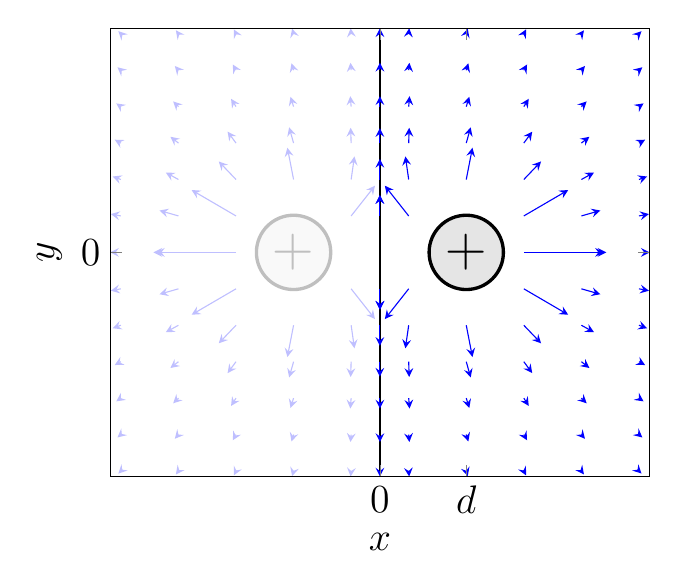
\begin{tikzpicture}[font=\Large]
  \begin{axis}[
    domain=-3:3,
    view={0}{90},
    axis background,
    xlabel={$x$},
    ylabel={$y$},
    xtick={0, 1},
    xticklabels={0, $d$},
    ytick={0},
  ]

    \pgfmathsetmacro{\arrowscale}{0.4} % Define the variable here
    \addplot3 [
        blue!25,-stealth,samples=5,
        quiver={
            u={(x-1)/((x-1)^2 + y^2)^(3/2) + (x+1)/((x+1)^2 + y^2)^(3/2)},
            v={(y)/((x-1)^2 + y^2)^(3/2) + (y)/((x+1)^2 + y^2)^(3/2)},
            scale arrows=\arrowscale,
        },
        domain = -1/3:-3,
        domain y = 1:3,
    ] {1};
    \addplot3 [
        blue!25,-stealth,samples=5,
        quiver={
            u={(x-1)/((x-1)^2 + y^2)^(3/2) + (x+1)/((x+1)^2 + y^2)^(3/2)},
            v={(y)/((x-1)^2 + y^2)^(3/2) + (y)/((x+1)^2 + y^2)^(3/2)},
            scale arrows=\arrowscale,
        },
        domain = -1/3:-3,
        domain y = -3:-1,
    ] {1};
    \addplot3 [
        blue!25,-stealth,samples=3,
        quiver={
            u={(x-1)/((x-1)^2 + y^2)^(3/2) + (x+1)/((x+1)^2 + y^2)^(3/2)},
            v={(y)/((x-1)^2 + y^2)^(3/2) + (y)/((x+1)^2 + y^2)^(3/2)},
            scale arrows=\arrowscale,
        },
        domain = -5/3:-3,
        domain y = -0.5:0.5,
    ] {1};
    \addplot3 [
        blue!25,-stealth,samples=2, samples y=2,
        quiver={
            u={(x-1)/((x-1)^2 + y^2)^(3/2) + (x+1)/((x+1)^2 + y^2)^(3/2)},
            v={(y)/((x-1)^2 + y^2)^(3/2) + (y)/((x+1)^2 + y^2)^(3/2)},
            scale arrows=\arrowscale,
        },
        domain = 0:-1/3,
        domain y = -0.5:0.5,
    ] {1};
    \node at (-1,0) [circle, draw=black!25, very thick, fill=gray!5, inner sep=2.5pt]{{\color{black!25}\huge{$+$}}};

    \draw[thick] (0,-3) -- (0,3);

    \addplot3 [
        blue,-stealth,samples=5,
        quiver={
            u={(x-1)/((x-1)^2 + y^2)^(3/2) + (x+1)/((x+1)^2 + y^2)^(3/2)},
            v={(y)/((x-1)^2 + y^2)^(3/2) + (y)/((x+1)^2 + y^2)^(3/2)},
            scale arrows=\arrowscale,
        },
        domain = 1/3:3,
        domain y = 1:3,
    ] {1};
    \addplot3 [
        blue,-stealth,samples=5,
        quiver={
            u={(x-1)/((x-1)^2 + y^2)^(3/2) + (x+1)/((x+1)^2 + y^2)^(3/2)},
            v={(y)/((x-1)^2 + y^2)^(3/2) + (y)/((x+1)^2 + y^2)^(3/2)},
            scale arrows=\arrowscale,
        },
        domain = 1/3:3,
        domain y = -3:-1,
    ] {1};
    \addplot3 [
        blue,-stealth,samples=3,
        quiver={
            u={(x-1)/((x-1)^2 + y^2)^(3/2) + (x+1)/((x+1)^2 + y^2)^(3/2)},
            v={(y)/((x-1)^2 + y^2)^(3/2) + (y)/((x+1)^2 + y^2)^(3/2)},
            scale arrows=\arrowscale,
        },
        domain = 5/3:3,
        domain y = -0.5:0.5,
    ] {1};
    \addplot3 [
        blue,-stealth,samples=2, samples y=2,
        quiver={
            u={(x-1)/((x-1)^2 + y^2)^(3/2) + (x+1)/((x+1)^2 + y^2)^(3/2)},
            v={(y)/((x-1)^2 + y^2)^(3/2) + (y)/((x+1)^2 + y^2)^(3/2)},
            scale arrows=\arrowscale,
        },
        domain = 0:1/3,
        domain y = -0.5:0.5,
    ] {1};
    \node at (1,0) [circle, draw=black, very thick, fill=gray!20, inner sep=2.5pt]{\huge{$+$}};

    \addplot [
        blue,
        quiver={
            u={(x-1)/((x-1)^2 + y^2)^(3/2) + (x+1)/((x+1)^2 + y^2)^(3/2)},
            v={(y)/((x-1)^2 + y^2)^(3/2) + (y)/((x+1)^2 + y^2)^(3/2)},
            scale arrows=\arrowscale,
        },
        -stealth,
    ] table {
        x y
        0 0.5 
        0 1 
        0 1.5 
        0 2
        0 2.5
        0 3
        0 -0.5 
        0 -1 
        0 -1.5 
        0 -2
        0 -2.5
        0 -3
    };
  \end{axis}

\end{tikzpicture}
\end{document}